\chapter{Implementation}
Our proposed obfuscator is made up of several components including an universal
Turing machine model implemented in C and several transformation passes based on
the LLVM compiler suite~\cite{LLVM}; As shown in \F~\ref{fig:five}, our Turing
obfuscator performs a three-phase process to generate the obfuscated output. The
first step translates both target program and universal Turing machine source code into LLVM
intermediate representation (IR). The obfuscator then iterates IR instructions
to identify obfuscation candidates (the second phase). Given all the
transformation candidates, we then perform the obfuscation transformation (the
third phase). The instrumented IR codes are further compiled into the final
executable output. We implement the universal Turing machine model with in total
580 lines of C code and LLVM passes with 341 lines of C++ code. We now
elaborate on each phase in details.

\begin{figure}
 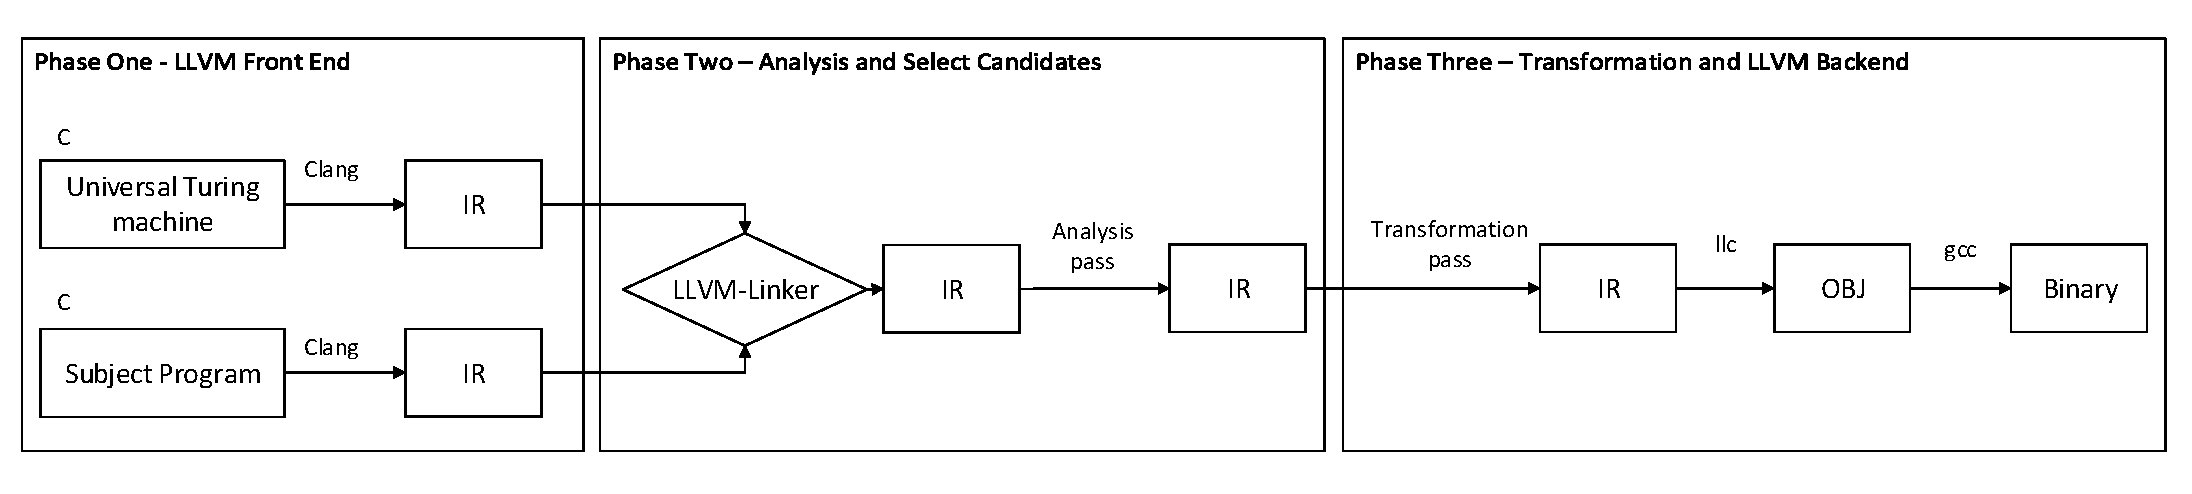
\includegraphics[width=\linewidth]{overview.pdf}
 \caption{Workflow of the Turing machine obfuscator.}
 \label{fig:five}
\end{figure}

\section{Phase One: Translate Source Code to IR}
\label{subsec:phase-one}
As aforementioned, we first compile the target source program into LLVM IR with
an appropriate LLVM front end compiler; the obfuscation transformation is
performed on the IR level. Considering a broad set of front end compilers
provided by LLVM which can turn programs written by various programming
languages into its IR, this IR-based implementation could broaden the
application scope our tool comparing with previous work~\cite{Ma, Zhi, Maieee}.
Since we employ C programs for the evaluation, Clang (version 5.0) is used as
the front end compiler in this thesis.

\section{Phase Two: Collect Transformation Candidate}
\label{subsec:phase-two}
The LLVM Pass framework is a core module of the LLVM compiler suite to conduct
analysis, transformation and optimization during the compile
time~\cite{LLVM}. We build a pass within this framework to iterate and
analyze every IR instruction in each module of the input program. During the
analysis pass, our Turing machine obfuscator locates all transformation
candidates on the IR instruction level.
\\\\
\noindent \textbf{Locate Candidate Predicates} While the proposed technique is
fundamentally capable of obfuscating any program component, the implementation
currently focuses on branch predicate since control-flow obfuscation is
efficient to defeat many reverse engineering activities
(\S\ref{sec:introduction}). In general, the transformation candidate set
includes 10 kinds of branch predicate instructions as: equal, not equal,
unsigned less than, unsigned greater than, unsigned less or equal, unsigned
greater or equal, signed less than, signed greater than, signed less or equal,
signed greater or equal.

\section{Phase Three: Obfuscation Transformation}
\label{subsec:phase-three}
The second phase provides all the eligible transformation candidates. We further
build another transformation pass within the LLVM Pass framework to perform the
obfuscation transformation. As shown in \F~\ref{fig:six}, predicate instructions
are obfuscated; we rewrite the instructions into function calls to the universal
Turing machine interface. The computation of the branch predicate is launched
inside the Turing machine, and the computation result is passed to a register
which directs the associated path selection. Our technique is able to obfuscate all the
branch predicates in a program or only transform a subset of (security
sensitive) candidates. Such partial obfuscation is denoted as ``obfuscation
level'' and we present discussion on this shortly.

\begin{figure}
 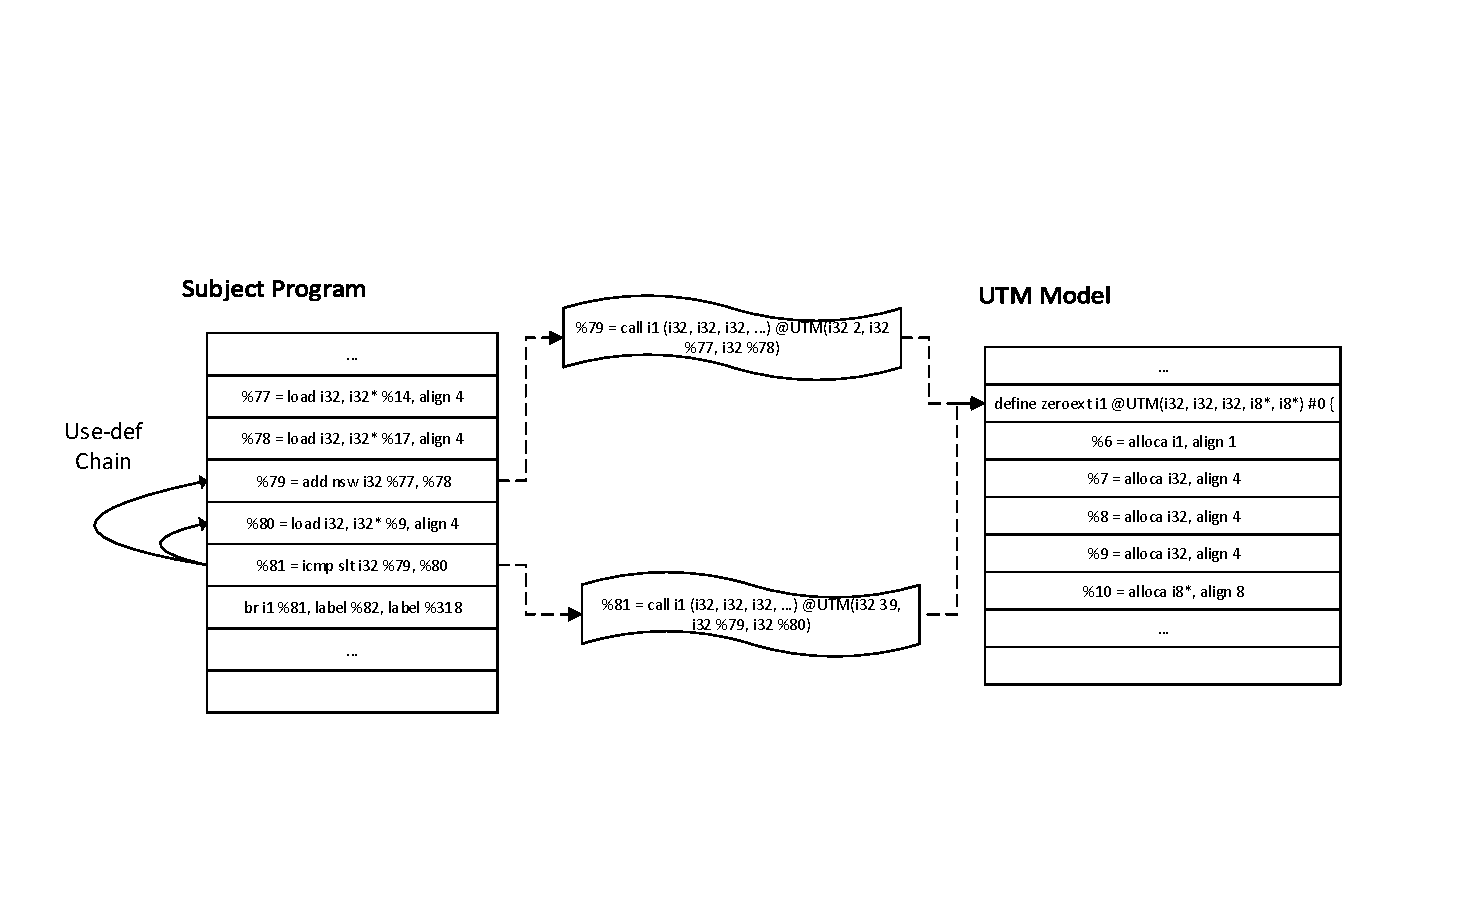
\includegraphics[width=\linewidth]{transform_pass.pdf}
 \caption{Obfuscation transformation for an \texttt{icmp} instruction. ``UTM''
   standards for universal Turing machine.}
 \label{fig:six}
\end{figure}

For an obfuscated predicate, our current ``transform to function call''
implementation utilizes the boolean return value to select a branch for control
transfer. On the other hand, we notice existing work (e.g., \cite{Ma, Maieee})
leverages a cross-procedure jump at this step; an indirect jump from the black
box of obfuscation component to a selected branch. We present further discussion on
both control transfer strategies in \S\ref{sec:discussion}.
%% \noindent \textbf{Negative Integer Operand Preprocess} In general, integer
%% operands comprise both positive and negative cases. Turing machine could only
%% dispose of positive operands in consequence of we use the length of dot cell on
%% tape to represent a integer. This means we have to preprocess the invalid
%% operands in Turing machine obfuscator. In the preprocessing stage, Turing
%% machine obfuscator could convert invalid operands to its opposite number to run
%% Turing machine. Calculate result from Turing machine is also revised before
%% returning. For instance, $-4 + (-6)$ is preprocessed to $4 + 6$, afterwards -10
%% which is the opposite number of 10 is returned. $4 + (-6)$ is preprocessed to
%% Turing machine operation $6 - 4$, and the opposite number of the outcome 2
%% (i.e., -2) is returned. In preprocess stage, any arithmetic operation would be
%% transformed to a valid integer operation with $+$, $-$, $\times$, $\div$ for
%% Turing machine.
\\\\
\noindent \textbf{Operand Type} In general, a branch predicate instruction can
have either pointer type or numerical data type (i.g., integer or float type).
While the proposed technique is generally capable of translating branch
predicate with any operand type, considering processing operands of pointer (and
float) type would bring in additional complexity, our current prototype is
designed to only handle operands of integer type. Actually our tentative study
shows that most of the branch predicate instructions would have operands of
integer type, hence, this implementation choice is indeed able to handle most of
the real-world cases. On the other hand, we emphasize there is no additional
research challenge to extend our technique to handle other cases. We leave it as
one future work to provide such functionalities.
\\\\
\noindent \textbf{Def-use Chain Analysis} Since our analysis is performed on IR
expressions of three-address form, one branch predicate in the original program
shall be translated into a sequence of IR instructions. Hence, to perform a
faithful obfuscation of one branch predicate, we need to first identify a
``region'' of IR instructions that is translated from this predicate.

As shown in \F\ref{fig:six}, we perform def-use analysis to recover such
``region'' information. In particular, given a comparison IR instruction (which
indicates one branch predicate and the end of the ``region''), we calculate the
use-def chains of its two operands, respectively. The identified instructions
which provide the ``definition'' information of these two operands will be
included in the ``region''. After the def-use analysis, we obfuscate all the
instructions in the ``region''.
\\\\
\noindent \textbf{Obfuscation Level} Obfuscation level is an indicator which
weighs how much of a program is transformed by the obfuscation pass. Consistent
with previous work (\cite{Trans}), the obfuscation level is defined as the ratio
between the obfuscated instruction and total eligible candidates:

\[ O = M / N \]

\(M\) is the number of instructions transformed by the obfuscation pass. \(N\)
is the number of all the transformable instructions (i.e., the branch predicate
instructions identified in \S~\ref{subsec:phase-two}).
